\documentclass[sigplan,review,fleqn]{acmart}
\usepackage{agda}

%% Rights management information.  This information is sent to you
%% when you complete the rights form.  These commands have SAMPLE
%% values in them; it is your responsibility as an author to replace
%% the commands and values with those provided to you when you
%% complete the rights form.
\setcopyright{rightsretained}
%\setcopyright{acmcopyright}
%\copyrightyear{2018}
%\acmYear{2018}
\acmISBN{}
\acmDOI{}

%%
%% These commands are for a JOURNAL article.
%\acmJournal{PACMPL}
%\acmVolume{0}
%\acmNumber{0}
%\acmArticle{0}
%\acmMonth{0}

\acmConference[TyDe'22]{Workshop on Type-Driven Development}{September 11, 2022}{Ljubljana, Slovenia}

%%
%% Submission ID.
%% Use this when submitting an article to a sponsored event. You'll
%% receive a unique submission ID from the organizers
%% of the event, and this ID should be used as the parameter to this command.
%%\acmSubmissionID{123-A56-BU3}

%%
%% The majority of ACM publications use numbered citations and
%% references.  The command \citestyle{authoryear} switches to the
%% "author year" style.
%%
%% If you are preparing content for an event
%% sponsored by ACM SIGGRAPH, you must use the "author year" style of
%% citations and references.
%% Uncommenting
%% the next command will enable that style.
\citestyle{acmauthoryear}
\setcitestyle{nosort}

\settopmatter{printacmref=false}

\usepackage[british]{babel}
%\usepackage[hyperpageref]{backref} % this may be removed

\usepackage{mathtools}
\usepackage[euler]{textgreek}

\usepackage[capitalise,noabbrev]{cleveref}
\usepackage{xifthen}
\newcommand{\varcitet}[3][]{\citeauthor{#2}#3~[\ifthenelse{\isempty{#1}}{\citeyear{#2}}{\citeyear[#1]{#2}}]}
\newcommand{\NoPeriod}[1]{\,}

\usepackage[color=yellow,textsize=scriptsize]{todonotes}
\setlength{\marginparwidth}{1.25cm}

\newcommand{\LT}[1]{\todo[author=LT,inline,color=green!40,caption={}]{{#1}}}
\newcommand{\Josh}[1]{\todo[author=Josh,inline,caption={}]{{#1}}}
\newcommand{\Viktor}[1]{\todo[author=Viktor,inline,color=orange,caption={}]{{#1}}}

\usepackage[inline]{enumitem} % for environment enumerate*

\captionsetup{aboveskip=1.5ex minus .5ex,belowskip=-1.5ex minus .5ex}
\newcommand{\codefigure}{\footnotesize\setlength{\mathindent}{0em}\setlength{\abovedisplayskip}{0ex}\setlength{\belowdisplayskip}{0ex}\noindent}

\newcommand{\arXiv}[1]{\href{http://arxiv.org/abs/#1}{arXiv:\nolinkurl{#1}}}

\let\Bbbk\relax
%% ODER: format ==         = "\mathrel{==}"
%% ODER: format /=         = "\neq "
%
%
\makeatletter
\@ifundefined{lhs2tex.lhs2tex.sty.read}%
  {\@namedef{lhs2tex.lhs2tex.sty.read}{}%
   \newcommand\SkipToFmtEnd{}%
   \newcommand\EndFmtInput{}%
   \long\def\SkipToFmtEnd#1\EndFmtInput{}%
  }\SkipToFmtEnd

\newcommand\ReadOnlyOnce[1]{\@ifundefined{#1}{\@namedef{#1}{}}\SkipToFmtEnd}
\usepackage{amstext}
\usepackage{amssymb}
\usepackage{stmaryrd}
\DeclareFontFamily{OT1}{cmtex}{}
\DeclareFontShape{OT1}{cmtex}{m}{n}
  {<5><6><7><8>cmtex8
   <9>cmtex9
   <10><10.95><12><14.4><17.28><20.74><24.88>cmtex10}{}
\DeclareFontShape{OT1}{cmtex}{m}{it}
  {<-> ssub * cmtt/m/it}{}
\newcommand{\texfamily}{\fontfamily{cmtex}\selectfont}
\DeclareFontShape{OT1}{cmtt}{bx}{n}
  {<5><6><7><8>cmtt8
   <9>cmbtt9
   <10><10.95><12><14.4><17.28><20.74><24.88>cmbtt10}{}
\DeclareFontShape{OT1}{cmtex}{bx}{n}
  {<-> ssub * cmtt/bx/n}{}
\newcommand{\tex}[1]{\text{\texfamily#1}}	% NEU

\newcommand{\Sp}{\hskip.33334em\relax}


\newcommand{\Conid}[1]{\mathit{#1}}
\newcommand{\Varid}[1]{\mathit{#1}}
\newcommand{\anonymous}{\kern0.06em \vbox{\hrule\@width.5em}}
\newcommand{\plus}{\mathbin{+\!\!\!+}}
\newcommand{\bind}{\mathbin{>\!\!\!>\mkern-6.7mu=}}
\newcommand{\rbind}{\mathbin{=\mkern-6.7mu<\!\!\!<}}% suggested by Neil Mitchell
\newcommand{\sequ}{\mathbin{>\!\!\!>}}
\renewcommand{\leq}{\leqslant}
\renewcommand{\geq}{\geqslant}
\usepackage{polytable}

%mathindent has to be defined
\@ifundefined{mathindent}%
  {\newdimen\mathindent\mathindent\leftmargini}%
  {}%

\def\resethooks{%
  \global\let\SaveRestoreHook\empty
  \global\let\ColumnHook\empty}
\newcommand*{\savecolumns}[1][default]%
  {\g@addto@macro\SaveRestoreHook{\savecolumns[#1]}}
\newcommand*{\restorecolumns}[1][default]%
  {\g@addto@macro\SaveRestoreHook{\restorecolumns[#1]}}
\newcommand*{\aligncolumn}[2]%
  {\g@addto@macro\ColumnHook{\column{#1}{#2}}}

\resethooks

\newcommand{\onelinecommentchars}{\quad-{}- }
\newcommand{\commentbeginchars}{\enskip\{-}
\newcommand{\commentendchars}{-\}\enskip}

\newcommand{\visiblecomments}{%
  \let\onelinecomment=\onelinecommentchars
  \let\commentbegin=\commentbeginchars
  \let\commentend=\commentendchars}

\newcommand{\invisiblecomments}{%
  \let\onelinecomment=\empty
  \let\commentbegin=\empty
  \let\commentend=\empty}

\visiblecomments

\newlength{\blanklineskip}
\setlength{\blanklineskip}{0.66084ex}

\newcommand{\hsindent}[1]{\quad}% default is fixed indentation
\let\hspre\empty
\let\hspost\empty
\newcommand{\NB}{\textbf{NB}}
\newcommand{\Todo}[1]{$\langle$\textbf{To do:}~#1$\rangle$}

\EndFmtInput
\makeatother
%
%
%
%
%
%
% This package provides two environments suitable to take the place
% of hscode, called "plainhscode" and "arrayhscode". 
%
% The plain environment surrounds each code block by vertical space,
% and it uses \abovedisplayskip and \belowdisplayskip to get spacing
% similar to formulas. Note that if these dimensions are changed,
% the spacing around displayed math formulas changes as well.
% All code is indented using \leftskip.
%
% Changed 19.08.2004 to reflect changes in colorcode. Should work with
% CodeGroup.sty.
%
\ReadOnlyOnce{polycode.fmt}%
\makeatletter

\newcommand{\hsnewpar}[1]%
  {{\parskip=0pt\parindent=0pt\par\vskip #1\noindent}}

% can be used, for instance, to redefine the code size, by setting the
% command to \small or something alike
\newcommand{\hscodestyle}{}

% The command \sethscode can be used to switch the code formatting
% behaviour by mapping the hscode environment in the subst directive
% to a new LaTeX environment.

\newcommand{\sethscode}[1]%
  {\expandafter\let\expandafter\hscode\csname #1\endcsname
   \expandafter\let\expandafter\endhscode\csname end#1\endcsname}

% "compatibility" mode restores the non-polycode.fmt layout.

\newenvironment{compathscode}%
  {\par\noindent
   \advance\leftskip\mathindent
   \hscodestyle
   \let\\=\@normalcr
   \let\hspre\(\let\hspost\)%
   \pboxed}%
  {\endpboxed\)%
   \par\noindent
   \ignorespacesafterend}

\newcommand{\compaths}{\sethscode{compathscode}}

% "plain" mode is the proposed default.
% It should now work with \centering.
% This required some changes. The old version
% is still available for reference as oldplainhscode.

\newenvironment{plainhscode}%
  {\hsnewpar\abovedisplayskip
   \advance\leftskip\mathindent
   \hscodestyle
   \let\hspre\(\let\hspost\)%
   \pboxed}%
  {\endpboxed%
   \hsnewpar\belowdisplayskip
   \ignorespacesafterend}

\newenvironment{oldplainhscode}%
  {\hsnewpar\abovedisplayskip
   \advance\leftskip\mathindent
   \hscodestyle
   \let\\=\@normalcr
   \(\pboxed}%
  {\endpboxed\)%
   \hsnewpar\belowdisplayskip
   \ignorespacesafterend}

% Here, we make plainhscode the default environment.

\newcommand{\plainhs}{\sethscode{plainhscode}}
\newcommand{\oldplainhs}{\sethscode{oldplainhscode}}
\plainhs

% The arrayhscode is like plain, but makes use of polytable's
% parray environment which disallows page breaks in code blocks.

\newenvironment{arrayhscode}%
  {\hsnewpar\abovedisplayskip
   \advance\leftskip\mathindent
   \hscodestyle
   \let\\=\@normalcr
   \(\parray}%
  {\endparray\)%
   \hsnewpar\belowdisplayskip
   \ignorespacesafterend}

\newcommand{\arrayhs}{\sethscode{arrayhscode}}

% The mathhscode environment also makes use of polytable's parray 
% environment. It is supposed to be used only inside math mode 
% (I used it to typeset the type rules in my thesis).

\newenvironment{mathhscode}%
  {\parray}{\endparray}

\newcommand{\mathhs}{\sethscode{mathhscode}}

% texths is similar to mathhs, but works in text mode.

\newenvironment{texthscode}%
  {\(\parray}{\endparray\)}

\newcommand{\texths}{\sethscode{texthscode}}

% The framed environment places code in a framed box.

\def\codeframewidth{\arrayrulewidth}
\RequirePackage{calc}

\newenvironment{framedhscode}%
  {\parskip=\abovedisplayskip\par\noindent
   \hscodestyle
   \arrayrulewidth=\codeframewidth
   \tabular{@{}|p{\linewidth-2\arraycolsep-2\arrayrulewidth-2pt}|@{}}%
   \hline\framedhslinecorrect\\{-1.5ex}%
   \let\endoflinesave=\\
   \let\\=\@normalcr
   \(\pboxed}%
  {\endpboxed\)%
   \framedhslinecorrect\endoflinesave{.5ex}\hline
   \endtabular
   \parskip=\belowdisplayskip\par\noindent
   \ignorespacesafterend}

\newcommand{\framedhslinecorrect}[2]%
  {#1[#2]}

\newcommand{\framedhs}{\sethscode{framedhscode}}

% The inlinehscode environment is an experimental environment
% that can be used to typeset displayed code inline.

\newenvironment{inlinehscode}%
  {\(\def\column##1##2{}%
   \let\>\undefined\let\<\undefined\let\\\undefined
   \newcommand\>[1][]{}\newcommand\<[1][]{}\newcommand\\[1][]{}%
   \def\fromto##1##2##3{##3}%
   \def\nextline{}}{\) }%

\newcommand{\inlinehs}{\sethscode{inlinehscode}}

% The joincode environment is a separate environment that
% can be used to surround and thereby connect multiple code
% blocks.

\newenvironment{joincode}%
  {\let\orighscode=\hscode
   \let\origendhscode=\endhscode
   \def\endhscode{\def\hscode{\endgroup\def\@currenvir{hscode}\\}\begingroup}
   %\let\SaveRestoreHook=\empty
   %\let\ColumnHook=\empty
   %\let\resethooks=\empty
   \orighscode\def\hscode{\endgroup\def\@currenvir{hscode}}}%
  {\origendhscode
   \global\let\hscode=\orighscode
   \global\let\endhscode=\origendhscode}%

\makeatother
\EndFmtInput
%
%
\ReadOnlyOnce{agda.fmt}%


\RequirePackage[T1]{fontenc}
\RequirePackage[utf8x]{inputenc}
\RequirePackage{ucs}
\RequirePackage{amsfonts}

\renewcommand{\ttdefault}{\sfdefault}
\usepackage{newverbs}
\renewcommand{\verb}{\collectverb{\color{AgdaFunction}}}
\newcommand{\con}{\collectverb{\color{AgdaInductiveConstructor}}}
\newcommand{\macro}{\collectverb{\color{AgdaMacro}}}
\newcommand{\name}{\collectverb{\it}}
\providecommand\mathbbm{\mathbb}

% TODO: Define more of these ...
\DeclareUnicodeCharacter{737}{\textsuperscript{l}}
\DeclareUnicodeCharacter{8718}{\ensuremath{\blacksquare}}
\DeclareUnicodeCharacter{8759}{::}
\DeclareUnicodeCharacter{9669}{\ensuremath{\triangleleft}}
\DeclareUnicodeCharacter{8799}{\ensuremath{\stackrel{\scriptscriptstyle ?}{=}}}
\DeclareUnicodeCharacter{10214}{\ensuremath{\llbracket}}
\DeclareUnicodeCharacter{10215}{\ensuremath{\rrbracket}}
\DeclareUnicodeCharacter{9632}{\ensuremath{\mathnormal\blacksquare}}
\DeclareUnicodeCharacter{7580}{\textsuperscript{c}}
\DeclareUnicodeCharacter{8245}{\ensuremath{^\backprime}}

% TODO: This is in general not a good idea.
\providecommand\textepsilon{$\epsilon$}
\providecommand\textmu{$\mu$}


%Actually, varsyms should not occur in Agda output.

% TODO: Make this configurable. IMHO, italics doesn't work well
% for Agda code.

\renewcommand\Varid[1]{\mathord{\textsf{#1}}}
\let\Conid\Varid
\newcommand\Keyword[1]{\textsf{\textbf{#1}}}
\EndFmtInput


\newcommand{\cons}[1]{\mathbf{#1}}
\newcommand{\iden}{\mathit}

\newcommand{\awa}[2]{\mathrlap{#2}\phantom{#1}} % as wide as

\usepackage{xcolor}
\definecolor{addition}{RGB}{204,255,216}
\newcommand{\highlight}[2]{\smash{\text{\colorbox{#1}{\kern-.1em\vphantom{\vrule height 1.2ex depth 0.1ex}\smash{\ensuremath{#2}}\kern-.1em}}}}

\usepackage{graphicx}

%%format ` = "{}^\backprime"
%%format `Set = ` Set
%%format `[] = ` []
%%format `∷ = "\mathop{" ` "{" ∷ "}}"










%%
%% end of the preamble, start of the body of the document source.
\begin{document}

\setlength{\mathindent}{.5\parindent}

%%
%% The "title" command has an optional parameter,
%% allowing the author to define a "short title" to be used in page headers.
\title{Syntax-Generic Operations, Reflectively Reified}
\subtitle{Extended Abstract}

%% the authors and their affiliations.
%% Of note is the shared affiliation of the first two authors, and the
%% "authornote" and "authornotemark" commands
%% used to denote shared contribution to the research.
\author{Tzu-Chi Lin}
\orcid{0000-0002-7656-6225}
\email{vik@iis.sinica.edu.tw}
\affiliation{%
	\institution{Institute of Information Science, Academia Sinica}
	\streetaddress{128 Academia Road, Section 2, Nankang}
	\city{Taipei}
	\country{Taiwan}
	\postcode{115201}
}

\author{Hsiang-Shang Ko}
\email{joshko@iis.sinica.edu.tw}
\orcid{0000-0002-2439-1048}
\affiliation{%
	\institution{Institute of Information Science, Academia Sinica}
	\streetaddress{128 Academia Road, Section 2, Nankang}
	\city{Taipei}
	\country{Taiwan}
	\postcode{115201}
}

%\author{Liang-Ting Chen}
%\email{liang.ting.chen.tw@gmail.com}
%\orcid{0000-0002-3250-1331}
%\affiliation{%
%	\institution{Institute of Information Science, Academia Sinica}
%	\streetaddress{128 Academia Road, Section 2, Nankang}
%	\city{Taipei}
%	\country{Taiwan}
%	\postcode{115201}
%}

%%
%% By default, the full list of authors will be used in the page
%% headers. Often, this list is too long, and will overlap
%% other information printed in the page headers. This command allows
%% the author to define a more concise list
%% of authors' names for this purpose.
%\renewcommand{\shortauthors}{Trovato and Tobin, et al.}

%\begin{CCSXML}
%<ccs2012>
%   <concept>
%       <concept_id>10011007.10011006.10011008.10011009.10011012</concept_id>
%       <concept_desc>Software and its engineering~Functional languages</concept_desc>
%       <concept_significance>500</concept_significance>
%       </concept>
%   <concept>
%       <concept_id>10003752.10003790.10011740</concept_id>
%       <concept_desc>Theory of computation~Type theory</concept_desc>
%       <concept_significance>100</concept_significance>
%       </concept>
%   <concept>
%       <concept_id>10011007.10011006.10011008.10011024.10011028</concept_id>
%       <concept_desc>Software and its engineering~Data types and structures</concept_desc>
%       <concept_significance>500</concept_significance>
%       </concept>
% </ccs2012>
%\end{CCSXML}
%
%\ccsdesc[500]{Software and its engineering~Functional languages}
%\ccsdesc[300]{Theory of computation~Type theory}
%\ccsdesc[300]{Software and its engineering~Data types and structures}
%
%\keywords{typed metaprogramming, datatype-generic programming, inductive families, ornaments}

\begin{abstract}
Libraries of generic operations on syntax trees with binders are emerging, and one of these is \varcitet{Allais-generic-syntax}{'s} datatype-generic library in Agda, which provides syntax-generic constructions but not in a conventional form preferred by programmers.
We port a core part of \citeauthor{Allais-generic-syntax}'s library to our new datatype-generic framework, which uses Agda's elaborator reflection to reify generic constructions to programs close to what programmers would write by hand.
We hope that this work will make syntax-generic libraries such as \citeauthor{Allais-generic-syntax}'s more attractive, and stimulate discussion on the development of such libraries.
\end{abstract}

\maketitle

\section{Introduction}
\label{sec:intro}
When implementing embedded domain-specific languages (DSLs), dependently typed programmers make use of the host languages' type systems to enforce properties of the syntaxes.
In particular, when the syntaxes have binders and are typed, intrinsic typing has become a standard technique to make the programs well scoped and typed~\citep[Part~2]{Kokke-PLFA}.
Such syntaxes share similar type structures, operations, and lemmas (with the simplest examples being renaming and substitution).
Traditionally, programmers need to somewhat tediously redefine the operations for every distinct syntax.
Recently, there have been generic libraries providing constructions that can be specialised for a whole family of syntaxes with binders~\citep{Allais-generic-syntax,Fiore-SOAS-Agda,Ahrens-typed-abstract-syntax}, although it remains to be seen whether these libraries will be widely adopted.

We will focus on \varcitet{Allais-generic-syntax}{'s} Agda library, which treats syntax-generic programs as special cases of \emph{datatype-generic} programs~\citep{Gibbons-DGP,Benke-generic-universes,Altenkirch-GP-within-DTP}.
%in the sense that syntaxes are typically defined as datatypes.
Their approach (recapped in \cref{sec:recap}) is more or less standard in Agda:
The syntax of a DSL is specified as a `description' \name|d |\verb|: Desc |\name|I|\/ (where \name|I|\/~is the type of the DSL types), from which a datatype \verb|Tm |\name|d|\/ of syntax trees is derived.
There is a \verb|semantics| operator that traverses the syntax trees to compute a result; the operator is parametrised by a \verb|Semantics| record, which specifies what computation to perform.
The library provides various \verb|Semantics| parametrised by~\name|d|, which act as syntax-generic programs, and can be instantiated with \verb|semantics| as operations on syntax trees of DSLs that can be described within the \verb|Desc| universe.

One potential problem that may prevent \citeauthor{Allais-generic-syntax}'s library (and in general,  libraries following the standard approach to datatype-genericity in Agda) from being widely adopted is the lack of interoperability:
Programmers using \citeauthor{Allais-generic-syntax}'s library are restricted to using datatypes of the form \verb|Tm |\name|d|, which are rather different from the kind of native datatypes that programmers would normally write; this prevents access to other datatype-generic libraries (which use their own universes instead of \verb|Desc|), and makes language and editor support for native datatypes (such as representation optimisations~\citep{Brady-inductive-families-indices} and interactive case-splitting) less effective.
The problem also arises for the operations instantiated with \verb|semantics|, which are not as easy to work with as the hand-written versions (in particular when the definitions need to be inspected).
To address the problem (for datatype-generic libraries in general), the present authors (together with Liang-Ting Chen) proposed an Agda framework~\citep{Ko-NDGP} which uses \emph{elaborator reflection}~\citep{Christiansen-elaborator-reflection} to reify generic constructions as native datatypes and functions close to hand-written forms.
With the framework, programmers can keep the conventional programming style, and replace some of the programs that had to be written by hand with similar-looking ones automatically generated from generic libraries.

Here we report (in \cref{sec:demo}) a small but successful experiment porting a core part of \citeauthor{Allais-generic-syntax}'s library to our framework, allowing programmers to write datatypes of syntaxes in conventional forms and then reify \citeauthor{Allais-generic-syntax}'s syntax-generic operations as natural-looking functions.
We will give a demo at the workshop and show that our framework can potentially make syntax-generic libraries such as \citeauthor{Allais-generic-syntax}'s more attractive to programmers.
Moreover, currently there are noticeable limitations of \citeauthor{Allais-generic-syntax}'s library and of our framework (discussed in \cref{sec:discussion}), which we hope will stimulate discussion on how the development of syntax-generic libraries can be pushed further.
Our code is available at \url{https://github.com/Zekt/Generic-Scoped-Syntax}.

%\citet{Ko-NDGP} have tackled similar problems in datatype-generic programming.
%They argue that current generic programs either suffer from lack of interoperability or inefficiency.
%Programmers who are in need of a universe of syntaxes would typically design one specifically for their intended usage, making it hard to carry a definition in a universe to the others.
%Also instantiated operations defined on least fixed points of endofunctors differ greatly in semblance and efficiency from their native counterparts.
%Existing syntaxes and operations need to be redefined for a specific universe in order to be interoperable.
%Thus Ko et al. provide a universe of datatypes of the host language (in their case, Agda), as well as the translations between instantiated generic programs and native ones via elaborator reflection (...).
%
%In this extended abstract, we reflect on
%1. how generic programs are defined on the syntax universe proposed by Allais et al.,
%2. how traditional syntax operations are defined,
%3. how our techniques, combined with utilities provided by Ko et al. can help DSL programmers, and
%4. give some examples and show our instantiation process of generic programs not only replace traditional generic programming, but also resemble native function definitions.

%1. relate the universe of syntaxes proposed by Allais et al. to the universe of datatypes proposed by Ko et al.,
%2. redefine syntax-generic programs from Allais et al. to generic programs on a subset of the datatype universe from Ko et al.,
%3. argue them to be equivalent in expressiveness, and
%4. give some examples.

%The universe we work on covers simply-typed languages with binders. \todo{Does it?}
%We see it as a demonstration of techniques that make DSL programmers and generic programmers' lives easier.
%Syntax-generic programmers can choose an arbitrary universe of syntax as long as it is proved to be a subset of the datatype universe.
%DSL programmers get to work on familiar native syntaxes, once they provide the proof of them belonging to some universes of syntaxes, generic operations defined on these universes can be instantiated via elaborator reflection.
%Such syntax operations and proofs are reified as native functions on native datatypes, making them interoperable with existing libraries.
%\todo{Why do we have to redefine on this universe?}

\section{Allais et al.'s Approach}
\label{sec:recap}
We take a glimpse of syntax-generic programs on the universe of syntaxes \verb|Desc| defined by Allais et al.
All definitions in this section are directly referenced from Allais et al.
\begin{code}
	\>[0]\AgdaKeyword{data}\AgdaSpace{}%
	\AgdaDatatype{Desc}\AgdaSpace{}%
	\AgdaSymbol{(}\AgdaBound{I}\AgdaSpace{}%
	\AgdaSymbol{:}\AgdaSpace{}%
	\AgdaPrimitive{Set}\AgdaSymbol{)}\AgdaSpace{}%
	\AgdaSymbol{:}\AgdaSpace{}%
	\AgdaPrimitive{Set₁}\AgdaSpace{}%
	\AgdaKeyword{where}\<%	
	\\
	\>[0][@{}l@{\AgdaIndent{0}}]%
	\>[2]\AgdaInductiveConstructor{σ}%
	\>[5]\AgdaSymbol{:}\AgdaSpace{}%
	\AgdaSymbol{(}\AgdaBound{A}\AgdaSpace{}%
	\AgdaSymbol{:}\AgdaSpace{}%
	\AgdaPrimitive{Set}\AgdaSymbol{)}\AgdaSpace{}%
	\AgdaSymbol{→}\AgdaSpace{}%
	\AgdaSymbol{(}\AgdaBound{A}\AgdaSpace{}%
	\AgdaSymbol{→}\AgdaSpace{}%
	\AgdaDatatype{Desc}\AgdaSpace{}%
	\AgdaBound{I}\AgdaSymbol{)}\AgdaSpace{}%
	\AgdaSymbol{→}\AgdaSpace{}%
	\AgdaDatatype{Desc}\AgdaSpace{}%
	\AgdaBound{I}\<%
	\\
	%
	\>[2]\AgdaInductiveConstructor{‵X}\AgdaSpace{}%
	\AgdaSymbol{:}\AgdaSpace{}%
	\AgdaDatatype{List}\AgdaSpace{}%
	\AgdaBound{I}\AgdaSpace{}%
	\AgdaSymbol{→}\AgdaSpace{}%
	\AgdaBound{I}\AgdaSpace{}%
	\AgdaSymbol{→}\AgdaSpace{}%
	\AgdaDatatype{Desc}\AgdaSpace{}%
	\AgdaBound{I}\AgdaSpace{}%
	\AgdaSymbol{→}\AgdaSpace{}%
	\AgdaDatatype{Desc}\AgdaSpace{}%
	\AgdaBound{I}\<%
	\\
	%
	\>[2]\AgdaInductiveConstructor{■}%
	\>[5]\AgdaSymbol{:}\AgdaSpace{}%
	\AgdaBound{I}\AgdaSpace{}%
	\AgdaSymbol{→}\AgdaSpace{}%
	\AgdaDatatype{Desc}\AgdaSpace{}%
	\AgdaBound{I}\<%
\end{code}
A \con|σ| describes any branching of the construction by a dependent sigma type, a \con|‵X| describes an occurrence of recursion of the syntax being defined by taking its index, and a \con|■| ends a description with the index of the constructed syntax.
The interpretation function \verb|⟦_⟧| determines what a description actually means, i.e. what is needed to construct a syntax given a description.
For example, a syntax of simply typed lambda calculus can be defined in this universe as \verb|STLC|.
\verb|‵STLC| corresponds to the choice of constructors if it is natively defined.
\begin{code}
\>[0]\AgdaKeyword{data}\AgdaSpace{}%
\AgdaDatatype{Type}\AgdaSpace{}%
\AgdaSymbol{:}\AgdaSpace{}%
\AgdaPrimitive{Set}\AgdaSpace{}%
\AgdaKeyword{where}\<%
\\
\>[0][@{}l@{\AgdaIndent{0}}]%
\>[2]\AgdaInductiveConstructor{α}\AgdaSpace{}%
\AgdaSymbol{:}\AgdaSpace{}%
\AgdaDatatype{Type}\<%
\\
%
\>[2]\AgdaOperator{\AgdaInductiveConstructor{\AgdaUnderscore{}‵→\AgdaUnderscore{}}}\AgdaSpace{}%
\AgdaSymbol{:}\AgdaSpace{}%
\AgdaDatatype{Type}\AgdaSpace{}%
\AgdaSymbol{→}\AgdaSpace{}%
\AgdaDatatype{Type}\AgdaSpace{}%
\AgdaSymbol{→}\AgdaSpace{}%
\AgdaDatatype{Type}\<%
\\
%
\\[\AgdaEmptyExtraSkip]%
\>[0]\AgdaKeyword{data}\AgdaSpace{}%
\AgdaDatatype{‵STLC}\AgdaSpace{}%
\AgdaSymbol{:}\AgdaSpace{}%
\AgdaPrimitive{Set}\AgdaSpace{}%
\AgdaKeyword{where}\<%
\\
\>[0][@{}l@{\AgdaIndent{0}}]%
\>[2]\AgdaInductiveConstructor{App}\AgdaSpace{}%
\AgdaInductiveConstructor{Lam}\AgdaSpace{}%
\AgdaSymbol{:}\AgdaSpace{}%
\AgdaDatatype{Type}\AgdaSpace{}%
\AgdaSymbol{→}\AgdaSpace{}%
\AgdaDatatype{Type}\AgdaSpace{}%
\AgdaSymbol{→}\AgdaSpace{}%
\AgdaDatatype{‵STLC}\<%
\\
%
\\[\AgdaEmptyExtraSkip]%
\>[0]\AgdaFunction{STLC}\AgdaSpace{}%
\AgdaSymbol{:}\AgdaSpace{}%
\AgdaDatatype{Desc}\AgdaSpace{}%
\AgdaDatatype{Type}\<%
\\
\>[0]\AgdaFunction{STLC}\AgdaSpace{}%
\AgdaSymbol{=}\AgdaSpace{}%
\AgdaInductiveConstructor{σ}\AgdaSpace{}%
\AgdaDatatype{‵STLC}\AgdaSpace{}%
\AgdaSymbol{λ}\AgdaSpace{}%
\AgdaKeyword{where}\<%
\\
\>[0][@{}l@{\AgdaIndent{0}}]%
\>[2]\AgdaSymbol{(}\AgdaInductiveConstructor{App}\AgdaSpace{}%
\AgdaBound{i}\AgdaSpace{}%
\AgdaBound{j}\AgdaSymbol{)}\AgdaSpace{}%
\AgdaSymbol{→}\AgdaSpace{}%
\AgdaInductiveConstructor{‵X}\AgdaSpace{}%
\AgdaInductiveConstructor{[]}\AgdaSpace{}%
\AgdaSymbol{(}\AgdaBound{i}\AgdaSpace{}%
\AgdaOperator{\AgdaInductiveConstructor{‵→}}\AgdaSpace{}%
\AgdaBound{j}\AgdaSymbol{)}\AgdaSpace{}%
\AgdaSymbol{(}\AgdaInductiveConstructor{‵X}\AgdaSpace{}%
\AgdaInductiveConstructor{[]}\AgdaSpace{}%
\AgdaBound{i}\AgdaSpace{}%
\AgdaSymbol{(}\AgdaInductiveConstructor{■}\AgdaSpace{}%
\AgdaBound{j}\AgdaSymbol{))}\<%
\\
%
\>[2]\AgdaSymbol{(}\AgdaInductiveConstructor{Lam}\AgdaSpace{}%
\AgdaBound{i}\AgdaSpace{}%
\AgdaBound{j}\AgdaSymbol{)}\AgdaSpace{}%
\AgdaSymbol{→}\AgdaSpace{}%
\AgdaInductiveConstructor{‵X}\AgdaSpace{}%
\AgdaSymbol{(}\AgdaBound{i}\AgdaSpace{}%
\AgdaOperator{\AgdaInductiveConstructor{∷}}\AgdaSpace{}%
\AgdaInductiveConstructor{[]}\AgdaSymbol{)}\AgdaSpace{}%
\AgdaBound{j}\AgdaSpace{}%
\AgdaSymbol{(}\AgdaInductiveConstructor{■}\AgdaSpace{}%
\AgdaSymbol{(}\AgdaBound{i}\AgdaSpace{}%
\AgdaOperator{\AgdaInductiveConstructor{‵→}}\AgdaSpace{}%
\AgdaBound{j}\AgdaSymbol{))}\<%
\end{code}
We can take the fixed points \verb|Tm| on which generic programs will operate.
For example, the term traversal functions of \verb|STLC| will operate on \verb|Tm STLC|.
\begin{code}
	\>[0]\AgdaKeyword{data}\AgdaSpace{}%
	\AgdaDatatype{Tm}\AgdaSpace{}%
	\AgdaSymbol{(}\AgdaBound{d}\AgdaSpace{}%
	\AgdaSymbol{:}\AgdaSpace{}%
	\AgdaDatatype{Desc}\AgdaSpace{}%
	\AgdaGeneralizable{I}\AgdaSymbol{)}\AgdaSpace{}%
	\AgdaSymbol{:}\AgdaSpace{}%
	\AgdaBound{I}\AgdaSpace{}%
	\AgdaSymbol{→}\AgdaSpace{}%
	\AgdaDatatype{List}\AgdaSpace{}%
	\AgdaBound{I}\AgdaSpace{}%
	\AgdaSymbol{→}\AgdaSpace{}%
	\AgdaPrimitive{Set}\<%
\end{code}

Allais et al. show that a subset of generic programs of term traversal can be described by \verb|Semantics|.
\verb|Semantics| is parametrised by a description and families \name|V| and \name|C| of type \name|I → |\verb|List|\name| I → |\verb|Set|.
\name|V| is the family of values that replaces bound variables during the traversal, and \name|C| is the family of what is computed from the traversal.
The actual term traversal function can be derived from a given \verb|Semantics| via the function \verb|semantics|.
\begin{code}
	\>[0]\AgdaKeyword{record}\AgdaSpace{}%
	\AgdaRecord{Semantics}\AgdaSpace{}%
	\AgdaSymbol{(}\AgdaBound{d}\AgdaSpace{}%
	\AgdaSymbol{:}\AgdaSpace{}%
	\AgdaDatatype{Desc}\AgdaSpace{}%
	\AgdaGeneralizable{I}\AgdaSymbol{)}\AgdaSpace{}%
	\AgdaSymbol{(}\AgdaBound{V}\AgdaSpace{}%
	\AgdaBound{C}\AgdaSpace{}%
	\AgdaSymbol{:}\AgdaSpace{}%
	\AgdaGeneralizable{I}\AgdaSpace{}%
	\AgdaSymbol{→}\AgdaSpace{}%
	\AgdaDatatype{List}\AgdaSpace{}%
	\AgdaGeneralizable{I}\AgdaSpace{}%
	\AgdaSymbol{→}\AgdaSpace{}%
	\AgdaPrimitive{Set}\AgdaSymbol{)}\AgdaSpace{}%
	\AgdaSymbol{:}\AgdaSpace{}%
	\AgdaPrimitive{Set}\<
	\\[\AgdaEmptyExtraSkip]%
	\\
	\>[0]\AgdaPostulate{semantics}%
	\>[226I]\AgdaSymbol{:}\AgdaSpace{}%
	\AgdaSymbol{∀}\AgdaSpace{}%
	\AgdaSymbol{\{}\AgdaBound{V}\AgdaSpace{}%
	\AgdaBound{C}\AgdaSpace{}%
	\AgdaSymbol{:}\AgdaSpace{}%
	\AgdaGeneralizable{I}\AgdaSpace{}%
	\AgdaSymbol{→}\AgdaSpace{}%
	\AgdaDatatype{List}\AgdaSpace{}%
	\AgdaGeneralizable{I}\AgdaSpace{}%
	\AgdaSymbol{→}\AgdaSpace{}%
	\AgdaPrimitive{Set}\AgdaSymbol{\}}\AgdaSpace{}%
	\AgdaSymbol{\{}\AgdaBound{d}\AgdaSpace{}%
	\AgdaSymbol{:}\AgdaSpace{}%
	\AgdaDatatype{Desc}\AgdaSpace{}%
	\AgdaGeneralizable{I}\AgdaSymbol{\}}\<%
	\\
	\>[.][@{}l@{}]\<[226I]%
	\>[10]\AgdaSymbol{→}\AgdaSpace{}%
	\AgdaRecord{Semantics}\AgdaSpace{}%
	\AgdaBound{d}\AgdaSpace{}%
	\AgdaBound{V}\AgdaSpace{}%
	\AgdaBound{C}\<%
	\\
	%
	\>[10]\AgdaSymbol{→}\AgdaSpace{}%
	\AgdaSymbol{(}\AgdaDatatype{Var}\AgdaSpace{}%
	\AgdaGeneralizable{i}\AgdaSpace{}%
	\AgdaGeneralizable{Γ}\AgdaSpace{}%
	\AgdaSymbol{→}\AgdaSpace{}%
	\AgdaBound{V}\AgdaSpace{}%
	\AgdaGeneralizable{i}\AgdaSpace{}%
	\AgdaGeneralizable{Δ}\AgdaSymbol{)}\<%
	\\
	%
	\>[10]\AgdaSymbol{→}\AgdaSpace{}%
	\AgdaSymbol{(∀}\AgdaSpace{}%
	\AgdaSymbol{\{}\AgdaBound{σ}\AgdaSymbol{\}}\AgdaSpace{}%
	\AgdaSymbol{→}\AgdaSpace{}%
	\AgdaDatatype{Tm}\AgdaSpace{}%
	\AgdaBound{d}\AgdaSpace{}%
	\AgdaBound{σ}\AgdaSpace{}%
	\AgdaGeneralizable{Γ}\AgdaSpace{}%
	\AgdaSymbol{→}\AgdaSpace{}%
	\AgdaBound{C}\AgdaSpace{}%
	\AgdaBound{σ}\AgdaSpace{}%
	\AgdaGeneralizable{Δ}\AgdaSymbol{)}\<%
\end{code}
The generic \verb|Semantics| of renaming \verb|Ren| (fig..) can be defined with \verb|Var| being values replacing bound variables and \verb|Tm|\name| d| being the computed result.
\begin{code}
	\>[0]\AgdaKeyword{data}\AgdaSpace{}%
	\AgdaDatatype{Var}\AgdaSpace{}%
	\AgdaSymbol{:}\AgdaSpace{}%
	\AgdaGeneralizable{I}\AgdaSpace{}%
	\AgdaSymbol{→}\AgdaSpace{}%
	\AgdaDatatype{List}\AgdaSpace{}%
	\AgdaGeneralizable{I}\AgdaSpace{}%
	\AgdaSymbol{→}\AgdaSpace{}%
	\AgdaPrimitive{Set}\AgdaSpace{}%
	\AgdaKeyword{where}\<%
	\\
	\>[0][@{}l@{\AgdaIndent{0}}]%
	\>[2]\AgdaInductiveConstructor{z}\AgdaSpace{}%
	\AgdaSymbol{:}\AgdaSpace{}%
	\AgdaDatatype{Var}\AgdaSpace{}%
	\AgdaGeneralizable{i}\AgdaSpace{}%
	\AgdaSymbol{(}\AgdaGeneralizable{i}\AgdaSpace{}%
	\AgdaOperator{\AgdaInductiveConstructor{∷}}\AgdaSpace{}%
	\AgdaGeneralizable{Γ}\AgdaSymbol{)}\<%
	\\
	%
	\>[2]\AgdaInductiveConstructor{s}\AgdaSpace{}%
	\AgdaSymbol{:}\AgdaSpace{}%
	\AgdaDatatype{Var}\AgdaSpace{}%
	\AgdaGeneralizable{i}\AgdaSpace{}%
	\AgdaGeneralizable{Γ}\AgdaSpace{}%
	\AgdaSymbol{→}\AgdaSpace{}%
	\AgdaDatatype{Var}\AgdaSpace{}%
	\AgdaGeneralizable{i}\AgdaSpace{}%
	\AgdaSymbol{(}\AgdaGeneralizable{j}\AgdaSpace{}%
	\AgdaOperator{\AgdaInductiveConstructor{∷}}\AgdaSpace{}%
	\AgdaGeneralizable{Γ}\AgdaSymbol{)}\<%
	\\
	\\[\AgdaEmptyExtraSkip]%
	\>[0]\AgdaPostulate{Ren}\AgdaSpace{}%
	\AgdaSymbol{:}\AgdaSpace{}%
	\AgdaRecord{Semantics}\AgdaSpace{}%
	\AgdaGeneralizable{d}\AgdaSpace{}%
	\AgdaDatatype{Var}\AgdaSpace{}%
	\AgdaSymbol{(}\AgdaDatatype{Tm}\AgdaSpace{}%
	\AgdaGeneralizable{d}\AgdaSymbol{)}\<%
\end{code}
To acquire the \verb|rename| function, one simply applies \verb|semantics| to \verb|Ren|.
\begin{code}
\>[0]\AgdaFunction{rename}\AgdaSpace{}%
\AgdaSymbol{:}\AgdaSpace{}%
\AgdaSymbol{(}\AgdaDatatype{Var}\AgdaSpace{}%
\AgdaGeneralizable{i}\AgdaSpace{}%
\AgdaGeneralizable{Γ}\AgdaSpace{}%
\AgdaSymbol{→}\AgdaSpace{}%
\AgdaDatatype{Var}\AgdaSpace{}%
\AgdaGeneralizable{i}\AgdaSpace{}%
\AgdaGeneralizable{Δ}\AgdaSymbol{)}\AgdaSpace{}
\AgdaSymbol{→}\AgdaSpace{}%
\AgdaDatatype{Tm}\AgdaSpace{}%
\AgdaBound{d}\AgdaSpace{}%
\AgdaBound{σ}\AgdaSpace{}%
\AgdaGeneralizable{Γ}\AgdaSpace{}%
\AgdaSymbol{→}\AgdaSpace{}%
\AgdaDatatype{Tm}\AgdaSpace{}%
\AgdaBound{d}\AgdaSpace{}%
\AgdaBound{σ}\AgdaSpace{}%
\AgdaGeneralizable{Δ}\<%
\\
\>[0]\AgdaFunction{rename}\AgdaSpace{}%
\AgdaBound{ρ}\AgdaSpace{}%
\AgdaBound{t}\AgdaSpace{}%
\AgdaSymbol{=}\AgdaSpace{}%
\AgdaPostulate{semantics}\AgdaSpace{}%
\AgdaPostulate{Ren}\AgdaSpace{}%
\AgdaBound{ρ}\AgdaSpace{}%
\AgdaBound{t}\<%
\end{code}
\verb|rename| is polymorphic so it is directly applicable to terms of \verb|STLC|, as the fixed point \verb|Tm|\name| d| will be instantiated to \verb|Tm STLC|. 


\section{Reifying Syntax-Generic Operations}
\label{sec:demo}
We have argued the benefits of native functions instead of those defined on a syntax universe in \cref{sec:intro}.
Therefore, we redefine constructions in \cref{sec:recap} such that every usage of the syntax universe are substituted with a datatype description \verb|DataD| along with a predicate \verb|Syntax|\name| : |\verb|DataD|\name| → |\verb|Set| that says a \verb|DataD| satisfies what is required for a datatype to be a syntax.
\verb|Semantics| and generic programs like \verb|Ren| in \cref{sec:recap} will be redefined in this section and have different types from their counterparts, despite playing similar roles.
We no longer need fixed points \verb|Tm| and \verb|semantics| which instantiates generic functions to \verb|Tm|.

We describe what a DSL programmer would typically program, then illustrate how they can exploit our library and metaprograms provided by Ko et al.

Take a DSL programmer who works on the datatype of syntax \verb|Lam| for example.
Traditionally, they would manually define a \verb|rename| function, as well as other syntax operations such as substitution, printer, or scope checker.
\begin{code}
	\>[0]\AgdaKeyword{data}\AgdaSpace{}%
	\AgdaDatatype{Lam}\AgdaSpace{}%
	\AgdaSymbol{:}\AgdaSpace{}%
	\AgdaDatatype{Type}\AgdaSpace{}%
	\AgdaSymbol{→}\AgdaSpace{}%
	\AgdaDatatype{List}\AgdaSpace{}%
	\AgdaDatatype{Type}\AgdaSpace{}%
	\AgdaSymbol{→}\AgdaSpace{}%
	\AgdaPrimitive{Set}\AgdaSpace{}%
	\AgdaKeyword{where}\<%
	\\
	\>[0][@{}l@{\AgdaIndent{0}}]%
	\>[2]\AgdaInductiveConstructor{‵var}\AgdaSpace{}%
	\AgdaSymbol{:}\AgdaSpace{}%
	\AgdaSymbol{∀}\AgdaSpace{}%
	\AgdaSymbol{\{}\AgdaBound{Γ}\AgdaSpace{}%
	\AgdaBound{σ}\AgdaSymbol{\}}%
	\>[19]\AgdaSymbol{→}\AgdaSpace{}%
	\AgdaDatatype{Var}\AgdaSpace{}%
	\AgdaBound{σ}\AgdaSpace{}%
	\AgdaBound{Γ}\AgdaSpace{}%
	\AgdaSymbol{→}\AgdaSpace{}%
	\AgdaDatatype{Lam}\AgdaSpace{}%
	\AgdaBound{σ}\AgdaSpace{}%
	\AgdaBound{Γ}\<%
	\\
	%
	\>[2]\AgdaInductiveConstructor{‵app}\AgdaSpace{}%
	\AgdaSymbol{:}\AgdaSpace{}%
	\AgdaSymbol{∀}\AgdaSpace{}%
	\AgdaSymbol{\{}\AgdaBound{Γ}\AgdaSpace{}%
	\AgdaBound{σ}\AgdaSpace{}%
	\AgdaBound{τ}\AgdaSymbol{\}}\AgdaSpace{}%
	\AgdaSymbol{→}\AgdaSpace{}%
	\AgdaDatatype{Lam}\AgdaSpace{}%
	\AgdaSymbol{(}\AgdaBound{σ}\AgdaSpace{}%
	\AgdaOperator{\AgdaInductiveConstructor{‵→}}\AgdaSpace{}%
	\AgdaBound{τ}\AgdaSymbol{)}\AgdaSpace{}%
	\AgdaBound{Γ}\AgdaSpace{}%
	\AgdaSymbol{→}\AgdaSpace{}%
	\AgdaDatatype{Lam}\AgdaSpace{}%
	\AgdaBound{σ}\AgdaSpace{}%
	\AgdaBound{Γ}\AgdaSpace{}%
	\AgdaSymbol{→}\AgdaSpace{}%
	\AgdaDatatype{Lam}\AgdaSpace{}%
	\AgdaBound{τ}\AgdaSpace{}%
	\AgdaBound{Γ}\<%
	\\
	%
	\>[2]\AgdaInductiveConstructor{‵lam}\AgdaSpace{}%
	\AgdaSymbol{:}\AgdaSpace{}%
	\AgdaSymbol{∀}\AgdaSpace{}%
	\AgdaSymbol{\{}\AgdaBound{Γ}\AgdaSpace{}%
	\AgdaBound{σ}\AgdaSpace{}%
	\AgdaBound{τ}\AgdaSymbol{\}}\AgdaSpace{}%
	\AgdaSymbol{→}\AgdaSpace{}%
	\AgdaDatatype{Lam}\AgdaSpace{}%
	\AgdaBound{τ}\AgdaSpace{}%
	\AgdaSymbol{(}\AgdaBound{σ}\AgdaSpace{}%
	\AgdaOperator{\AgdaInductiveConstructor{∷}}\AgdaSpace{}%
	\AgdaBound{Γ}\AgdaSymbol{)}%
	\>[36]\AgdaSymbol{→}\AgdaSpace{}%
	\AgdaDatatype{Lam}\AgdaSpace{}%
	\AgdaSymbol{(}\AgdaBound{σ}\AgdaSpace{}%
	\AgdaOperator{\AgdaInductiveConstructor{‵→}}\AgdaSpace{}%
	\AgdaBound{τ}\AgdaSymbol{)}\AgdaSpace{}%
	\AgdaBound{Γ}\<%
	\\
	\\[\AgdaEmptyExtraSkip]%
	\>[0]\AgdaFunction{extend}%
	\>[274I]\AgdaSymbol{:}\AgdaSpace{}%
	\AgdaSymbol{(∀}\AgdaSpace{}%
	\AgdaSymbol{\{}\AgdaBound{i}\AgdaSymbol{\}}\AgdaSpace{}%
	\AgdaSymbol{→}\AgdaSpace{}%
	\AgdaDatatype{Var}\AgdaSpace{}%
	\AgdaBound{i}\AgdaSpace{}%
	\AgdaGeneralizable{Γ}\AgdaSpace{}%
	\AgdaSymbol{→}\AgdaSpace{}%
	\AgdaDatatype{Var}\AgdaSpace{}%
	\AgdaBound{i}\AgdaSpace{}%
	\AgdaGeneralizable{Δ}\AgdaSymbol{)}\<%
	\\
	\>[.][@{}l@{}]\<[274I]%
	\>[7]\AgdaSymbol{→}\AgdaSpace{}%
	\AgdaDatatype{Var}\AgdaSpace{}%
	\AgdaGeneralizable{i}\AgdaSpace{}%
	\AgdaSymbol{(}\AgdaGeneralizable{j}\AgdaSpace{}%
	\AgdaOperator{\AgdaInductiveConstructor{∷}}\AgdaSpace{}%
	\AgdaGeneralizable{Γ}\AgdaSymbol{)}\AgdaSpace{}%
	\AgdaSymbol{→}\AgdaSpace{}%
	\AgdaDatatype{Var}\AgdaSpace{}%
	\AgdaGeneralizable{i}\AgdaSpace{}%
	\AgdaSymbol{(}\AgdaGeneralizable{j}\AgdaSpace{}%
	\AgdaOperator{\AgdaInductiveConstructor{∷}}\AgdaSpace{}%
	\AgdaGeneralizable{Δ}\AgdaSymbol{)}\<%
	\\
	\>[0]\AgdaFunction{extend}\AgdaSpace{}%
	\AgdaBound{f}\AgdaSpace{}%
	\AgdaInductiveConstructor{z}\AgdaSpace{}%
	\AgdaSymbol{=}\AgdaSpace{}%
	\AgdaInductiveConstructor{z}\<%
	\\
	\>[0]\AgdaFunction{extend}\AgdaSpace{}%
	\AgdaBound{f}\AgdaSpace{}%
	\AgdaSymbol{(}\AgdaInductiveConstructor{s}\AgdaSpace{}%
	\AgdaBound{v}\AgdaSymbol{)}\AgdaSpace{}%
	\AgdaSymbol{=}\AgdaSpace{}%
	\AgdaInductiveConstructor{s}\AgdaSpace{}%
	\AgdaSymbol{(}\AgdaBound{f}\AgdaSpace{}%
	\AgdaBound{v}\AgdaSymbol{)}\<%
	\\
	%
	\\[\AgdaEmptyExtraSkip]%
	\>[0]\AgdaFunction{rename}%
	\>[307I]\AgdaSymbol{:}\AgdaSpace{}%
	\AgdaSymbol{(∀}\AgdaSpace{}%
	\AgdaSymbol{\{}\AgdaBound{i}\AgdaSymbol{\}}\AgdaSpace{}%
	\AgdaSymbol{→}\AgdaSpace{}%
	\AgdaDatatype{Var}\AgdaSpace{}%
	\AgdaBound{i}\AgdaSpace{}%
	\AgdaGeneralizable{Γ}\AgdaSpace{}%
	\AgdaSymbol{→}\AgdaSpace{}%
	\AgdaDatatype{Var}\AgdaSpace{}%
	\AgdaBound{i}\AgdaSpace{}%
	\AgdaGeneralizable{Δ}\AgdaSymbol{)}\<%
	\\
	\>[.][@{}l@{}]\<[307I]%
	\>[7]\AgdaSymbol{→}\AgdaSpace{}%
	\AgdaDatatype{Lam}\AgdaSpace{}%
	\AgdaGeneralizable{j}\AgdaSpace{}%
	\AgdaGeneralizable{Γ}\AgdaSpace{}%
	\AgdaSymbol{→}\AgdaSpace{}%
	\AgdaDatatype{Lam}\AgdaSpace{}%
	\AgdaGeneralizable{j}\AgdaSpace{}%
	\AgdaGeneralizable{Δ}\<%
	\\
	\>[0]\AgdaFunction{rename}\AgdaSpace{}%
	\AgdaBound{f}\AgdaSpace{}%
	\AgdaSymbol{(}\AgdaInductiveConstructor{‵var}\AgdaSpace{}%
	\AgdaBound{x}\AgdaSymbol{)}%
	\>[20]\AgdaSymbol{=}\AgdaSpace{}%
	\AgdaInductiveConstructor{‵var}\AgdaSpace{}%
	\AgdaSymbol{(}\AgdaBound{f}\AgdaSpace{}%
	\AgdaBound{x}\AgdaSymbol{)}\<%
	\\
	\>[0]\AgdaFunction{rename}\AgdaSpace{}%
	\AgdaBound{f}\AgdaSpace{}%
	\AgdaSymbol{(}\AgdaInductiveConstructor{‵app}\AgdaSpace{}%
	\AgdaBound{x}\AgdaSpace{}%
	\AgdaBound{y}\AgdaSymbol{)}\AgdaSpace{}%
	\AgdaSymbol{=}\AgdaSpace{}%
	\AgdaInductiveConstructor{‵app}\AgdaSpace{}%
	\AgdaSymbol{(}\AgdaFunction{rename}\AgdaSpace{}%
	\AgdaBound{f}\AgdaSpace{}%
	\AgdaBound{x}\AgdaSymbol{)}\AgdaSpace{}%
	\AgdaSymbol{(}\AgdaFunction{rename}\AgdaSpace{}%
	\AgdaBound{f}\AgdaSpace{}%
	\AgdaBound{y}\AgdaSymbol{)}\<%
	\\
	\>[0]\AgdaFunction{rename}\AgdaSpace{}%
	\AgdaBound{f}\AgdaSpace{}%
	\AgdaSymbol{(}\AgdaInductiveConstructor{‵lam}\AgdaSpace{}%
	\AgdaBound{x}\AgdaSymbol{)}%
	\>[20]\AgdaSymbol{=}\AgdaSpace{}%
	\AgdaInductiveConstructor{‵lam}\AgdaSpace{}%
	\AgdaSymbol{(}\AgdaFunction{rename}\AgdaSpace{}%
	\AgdaSymbol{(}\AgdaFunction{extend}\AgdaSpace{}%
	\AgdaBound{f}\AgdaSymbol{)}\AgdaSpace{}%
	\AgdaBound{x}\AgdaSymbol{)}\<%
\end{code}
We show that these operations can be generated at once and the programmers need not redefine them for every new syntax.
More specifically, the \verb|rename| function generated by our utilities will be definitionally equivalent to the one the programmer manually defined.

The DSL programmer needs to provide a proof \verb|LamSyntax|\name| : |\verb|Syntax LamD| where \verb|LamD| is the datatype description of \verb|Lam|. 
Ko et al. have provided a macro \macro|genDataD| that generates from a native datatype its description of type \verb|DataD|.
\begin{code}
	\>[0]\AgdaFunction{LamD}\AgdaSpace{}%
	\AgdaSymbol{=}\AgdaSpace{}%
	\AgdaMacro{genDataD}\AgdaSpace{}%
	\AgdaDatatype{Lam}\<%
\end{code}
%This means that the programmer needs to have a basic understanding of \verb|DataD|. \todo{Discussion? DataD closely resemble native datatype definition in Agda.}
%More specifically, the core part of \verb|DataD|, \verb|ConDs| is a list in which each \verb|ConD| represents a constructor.
Now the programmer get to choose what generic syntax operation they want to instantiate.
For example, our library provides \verb|Renaming| that generates a \verb|Semantics| from a \name|D : |\verb|DataD| and its \verb|Syntax|\name| D|. 
\begin{code}
	\>[2]\AgdaPostulate{Renaming}%
	\>[296I]\AgdaSymbol{:}\AgdaSpace{}%
	\AgdaSymbol{(}\AgdaBound{D}\AgdaSpace{}%
	\AgdaSymbol{:}\AgdaSpace{}%
	\AgdaRecord{DataD}\AgdaSymbol{)}\<%
	\\
	\>[.][@{}l@{}]\<[296I]%
	\>[11]\AgdaSymbol{→}\AgdaSpace{}%
	\AgdaSymbol{(}\AgdaBound{Sy}\AgdaSpace{}%
	\AgdaSymbol{:}\AgdaSpace{}%
	\AgdaPostulate{Syntax}\AgdaSpace{}%
	\AgdaBound{D}\AgdaSymbol{)}\<%
	\\
	%
	\>[11]\AgdaSymbol{→}\AgdaSpace{}%
	\AgdaRecord{Semantics}\AgdaSpace{}%
	\AgdaBound{D}\AgdaSpace{}%
	\AgdaBound{Sy}\AgdaSpace{}%
	\AgdaDatatype{Var}\AgdaSpace{}%
	\AgdaDatatype{Lam}\<%
	\\
	\\[\AgdaEmptyExtraSkip]%
	\>[0]\AgdaFunction{LamSemantics}\AgdaSpace{}%
	\AgdaSymbol{=}\AgdaSpace{}%
	\AgdaPostulate{Renaming}\AgdaSpace{}%
	\AgdaFunction{LamD}\AgdaSpace{}%
	\AgdaPostulate{LamSyntax}\<%
\end{code}
We also provide a function \verb|SemP| that takes a datatype description, its proof of being syntax, and the \verb|Semantics| we just generated, then generates an instance of \verb|FoldP|.
\begin{code}
	\>[2]\AgdaPostulate{SemP}%
	\>[309I]\AgdaSymbol{:}\AgdaSpace{}%
	\AgdaSymbol{(}\AgdaBound{D}\AgdaSpace{}%
	\AgdaSymbol{:}\AgdaSpace{}%
	\AgdaRecord{DataD}\AgdaSymbol{)}\<%
	\\
	\>[.][@{}l@{}]\<[309I]%
	\>[7]\AgdaSymbol{→}\AgdaSpace{}%
	\AgdaSymbol{(}\AgdaBound{Sy}\AgdaSpace{}%
	\AgdaSymbol{:}\AgdaSpace{}%
	\AgdaPostulate{Syntax}\AgdaSpace{}%
	\AgdaBound{D}\AgdaSymbol{)}\<%
	\\
	%
	\>[7]\AgdaSymbol{→}\AgdaSpace{}%
	\AgdaRecord{Semantics}\AgdaSpace{}%
	\AgdaBound{D}\AgdaSpace{}%
	\AgdaBound{Sy}\AgdaSpace{}%
	\AgdaDatatype{Var}\AgdaSpace{}%
	\AgdaDatatype{Lam}\<%
	\\
	%
	\>[7]\AgdaSymbol{→}\AgdaSpace{}%
	\AgdaRecord{FoldP}\<%
	\\
	\\[\AgdaEmptyExtraSkip]%
	\>[0]\AgdaFunction{RenameP}\AgdaSpace{}%
	\AgdaSymbol{=}\AgdaSpace{}%
	\AgdaPostulate{SemP}\AgdaSpace{}%
	\AgdaSymbol{(}\AgdaMacro{genDataD}\AgdaSpace{}%
	\AgdaDatatype{Lam}\AgdaSymbol{)}\AgdaSpace{}%
	\AgdaPostulate{LamSyntax}\AgdaSpace{}%
	\AgdaFunction{LamSemantics}\<%
\end{code}
\verb|FoldP| and the metaprogram \verb|defineFold| are given by Ko et al., the former is the description of generic fold operations, and the latter instantiate them to native fold functions.
\begin{code}
	\>[0]\AgdaKeyword{unquoteDecl}\AgdaSpace{}%
	\AgdaDatatype{rename}\AgdaSpace{}%
	\AgdaSymbol{=}\AgdaSpace{}%
	\AgdaFunction{defineFold}\AgdaSpace{}%
	\AgdaFunction{RenameP}\AgdaSpace{}%
	\AgdaDatatype{rename}\<%
\end{code}
\AgdaKeyword{unquoteDecl} is a built-in primitive provided by Agda that defines a given name, in this case \verb|rename|, by a metaprogram.
Generated functions are scope- and type-checked, which means here a \verb|rename| function is immediately usable by the programmer.
Its definition is printed to Agda's debug buffer for the programmers to modify and replace the \AgdaKeyword{unquoteDecl} declaration with.    

The steps described can be summarized by \cref{fig:flow}. 
Macros and intermediate functions are represented in boxes, constructions that are generated and passed around are represented in arrows.
Solid arrows means native function application in Agda, where dotted arrows means they are generated by macros via elaborator reflection.

The programmer need not understand the details of the structures we just mentioned, except the datatype description \verb|DataD| and the proof of \verb|Syntax| they need to provide.
With the help of these utilities, we have shown that a DSL programmer only needs to prove their datatypes to be syntaxes to acquire instantiation of generic renaming, as well as other term traversal operations.
Delightfully they will find these operations are reified as native functions, close to what they would have written for the syntaxes they just defined.

\begin{figure}
	\centering
	\fbox{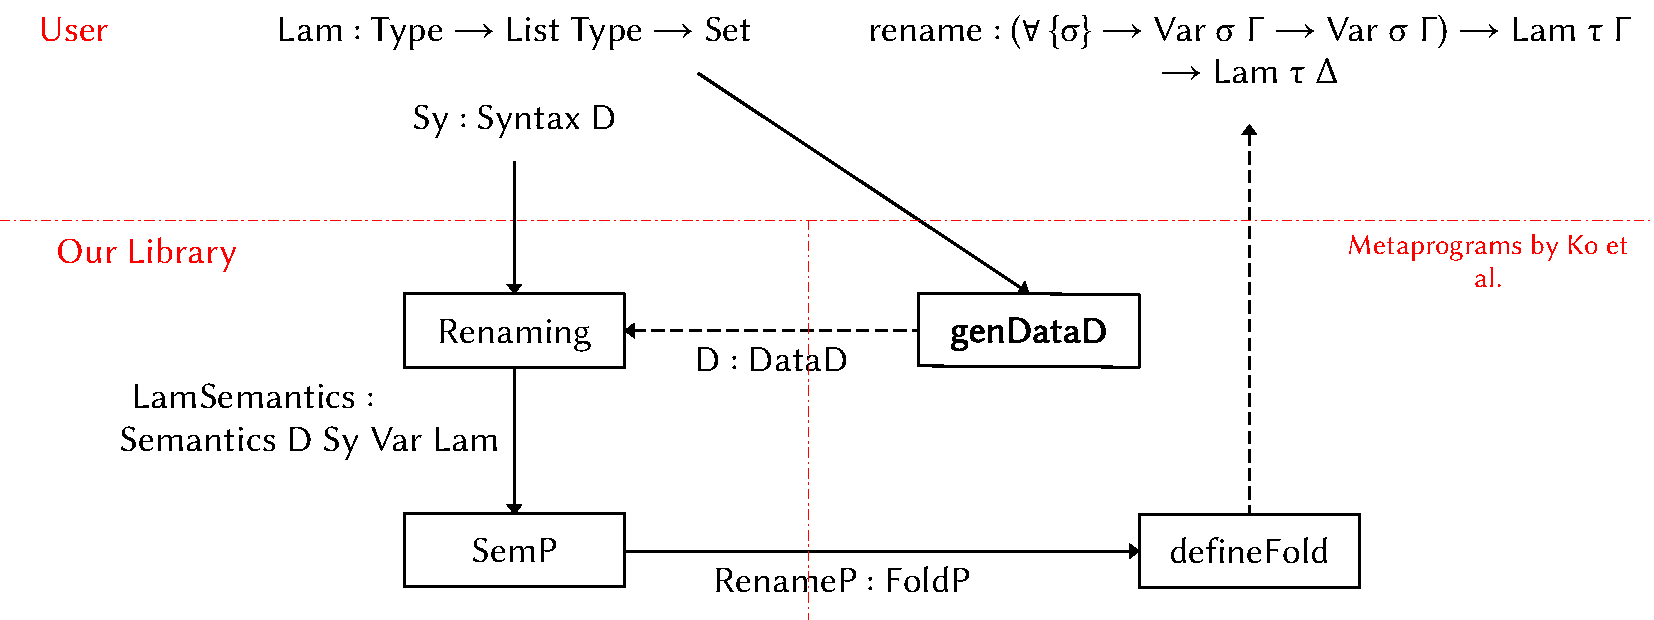
\includegraphics[width=\columnwidth]{Diagram}}
	\caption{An illustration of how a DSL programmer interact with our library and metaprograms by Ko et al.}
	\label{fig:flow}
\end{figure}

%\section{Behind the scenes}
%This section is more technical.
%We show how we redefine the constructions in \cref{sec:recap} on the universe of datatypes from Ko et al.
%
%We take a look at the datatype universe.
%\verb|ConDs| covers the representation for datatype constructors, each of which is described by a \verb|ConD|.
%A \verb|ConD| describes a single constructor as close to a Agda datatype constructor as possible.
%A \con|σ| describes a field of of the constructor with shallow embedding that takes any \verb|Set|, a \con|ρ| combined with \verb|RecD| describes a possibly higher-order recursion, a \con|ι| ends a description with the index of the constructed datatype.
%Notice the similarities and dissimilarities between \verb|Desc| and \verb|ConDs|, the latter is the gap which our predicates should fill in. 
%\begin{code}
%	\>[0]\AgdaKeyword{data}\AgdaSpace{}%
%	\AgdaDatatype{RecD}\AgdaSpace{}%
%	\AgdaSymbol{(}\AgdaBound{I}\AgdaSpace{}%
%	\AgdaSymbol{:}\AgdaSpace{}%
%	\AgdaPrimitive{Set}\AgdaSymbol{)}\AgdaSpace{}%
%	\AgdaSymbol{:}\AgdaSpace{}%
%	\AgdaPrimitive{Set₁}\AgdaSpace{}%
%	\AgdaKeyword{where}\<%
%	\\
%	\>[0][@{}l@{\AgdaIndent{0}}]%
%	\>[2]\AgdaInductiveConstructor{ι}\AgdaSpace{}%
%	\AgdaSymbol{:}\AgdaSpace{}%
%	\AgdaSymbol{(}\AgdaBound{i}\AgdaSpace{}%
%	\AgdaSymbol{:}\AgdaSpace{}%
%	\AgdaBound{I}\AgdaSymbol{)}\AgdaSpace{}%
%	\AgdaSymbol{→}\AgdaSpace{}%
%	\AgdaDatatype{RecD}\AgdaSpace{}%
%	\AgdaBound{I}\<%
%	\\
%	%
%	\>[2]\AgdaInductiveConstructor{π}\AgdaSpace{}%
%	\AgdaSymbol{:}\AgdaSpace{}%
%	\AgdaSymbol{(}\AgdaBound{A}\AgdaSpace{}%
%	\AgdaSymbol{:}\AgdaSpace{}%
%	\AgdaPrimitive{Set}\AgdaSymbol{)}\AgdaSpace{}%
%	\AgdaSymbol{(}\AgdaBound{D}\AgdaSpace{}%
%	\AgdaSymbol{:}\AgdaSpace{}%
%	\AgdaBound{A}\AgdaSpace{}%
%	\AgdaSymbol{→}\AgdaSpace{}%
%	\AgdaDatatype{RecD}\AgdaSpace{}%
%	\AgdaBound{I}\AgdaSymbol{)}\AgdaSpace{}%
%	\AgdaSymbol{→}\AgdaSpace{}%
%	\AgdaDatatype{RecD}\AgdaSpace{}%
%	\AgdaBound{I}\<%
%	\\
%	%
%	\\[\AgdaEmptyExtraSkip]%
%	\>[0]\AgdaKeyword{data}\AgdaSpace{}%
%	\AgdaDatatype{ConD}\AgdaSpace{}%
%	\AgdaSymbol{(}\AgdaBound{I}\AgdaSpace{}%
%	\AgdaSymbol{:}\AgdaSpace{}%
%	\AgdaPrimitive{Set}\AgdaSymbol{)}\AgdaSpace{}%
%	\AgdaSymbol{:}\AgdaSpace{}%
%	\AgdaPrimitive{Set₁}\AgdaSpace{}%
%	\AgdaKeyword{where}\<%
%	\\
%	\>[0][@{}l@{\AgdaIndent{0}}]%
%	\>[2]\AgdaInductiveConstructor{ι}\AgdaSpace{}%
%	\AgdaSymbol{:}\AgdaSpace{}%
%	\AgdaSymbol{(}\AgdaBound{i}\AgdaSpace{}%
%	\AgdaSymbol{:}\AgdaSpace{}%
%	\AgdaBound{I}\AgdaSymbol{)}\AgdaSpace{}%
%	\AgdaSymbol{→}\AgdaSpace{}%
%	\AgdaDatatype{ConD}\AgdaSpace{}%
%	\AgdaBound{I}\<%
%	\\
%	%
%	\>[2]\AgdaInductiveConstructor{σ}\AgdaSpace{}%
%	\AgdaSymbol{:}\AgdaSpace{}%
%	\AgdaSymbol{(}\AgdaBound{A}\AgdaSpace{}%
%	\AgdaSymbol{:}\AgdaSpace{}%
%	\AgdaPrimitive{Set}\AgdaSymbol{)}\AgdaSpace{}%
%	\AgdaSymbol{(}\AgdaBound{D}\AgdaSpace{}%
%	\AgdaSymbol{:}\AgdaSpace{}%
%	\AgdaBound{A}\AgdaSpace{}%
%	\AgdaSymbol{→}\AgdaSpace{}%
%	\AgdaDatatype{ConD}\AgdaSpace{}%
%	\AgdaBound{I}\AgdaSymbol{)}\AgdaSpace{}%
%	\AgdaSymbol{→}\AgdaSpace{}%
%	\AgdaDatatype{ConD}\AgdaSpace{}%
%	\AgdaBound{I}\<%
%	\\
%	%
%	\>[2]\AgdaInductiveConstructor{ρ}\AgdaSpace{}%
%	\AgdaSymbol{:}\AgdaSpace{}%
%	\AgdaSymbol{(}\AgdaBound{D}\AgdaSpace{}%
%	\AgdaSymbol{:}\AgdaSpace{}%
%	\AgdaDatatype{RecD}\AgdaSpace{}%
%	\AgdaBound{I}\AgdaSymbol{)}\AgdaSpace{}%
%	\AgdaSymbol{(}\AgdaBound{E}\AgdaSpace{}%
%	\AgdaSymbol{:}\AgdaSpace{}%
%	\AgdaDatatype{ConD}\AgdaSpace{}%
%	\AgdaBound{I}\AgdaSymbol{)}\AgdaSpace{}%
%	\AgdaSymbol{→}\AgdaSpace{}%
%	\AgdaDatatype{ConD}\AgdaSpace{}%
%	\AgdaBound{I}\<%
%	\\
%	%
%	\\[\AgdaEmptyExtraSkip]%
%	\>[0]\AgdaKeyword{data}\AgdaSpace{}%
%	\AgdaDatatype{ConDs}\AgdaSpace{}%
%	\AgdaSymbol{(}\AgdaBound{I}\AgdaSpace{}%
%	\AgdaSymbol{:}\AgdaSpace{}%
%	\AgdaPrimitive{Set}\AgdaSymbol{)}\AgdaSpace{}%
%	\AgdaSymbol{:}\AgdaSpace{}%
%	\AgdaPrimitive{Set₁}\AgdaSpace{}%
%	\AgdaKeyword{where}\<%
%	\\
%	\>[0][@{}l@{\AgdaIndent{0}}]%
%	\>[2]\AgdaInductiveConstructor{[]}%
%	\>[6]\AgdaSymbol{:}\AgdaSpace{}%
%	\AgdaDatatype{ConDs}\AgdaSpace{}%
%	\AgdaBound{I}\<%
%	\\
%	%
%	\>[2]\AgdaOperator{\AgdaInductiveConstructor{\AgdaUnderscore{}∷\AgdaUnderscore{}}}\AgdaSpace{}%
%	\AgdaSymbol{:}\AgdaSpace{}%
%	\AgdaSymbol{(}\AgdaBound{D}\AgdaSpace{}%
%	\AgdaSymbol{:}\AgdaSpace{}%
%	\AgdaDatatype{ConD}\AgdaSpace{}%
%	\AgdaBound{I}\AgdaSymbol{)}\AgdaSpace{}%
%	\AgdaSymbol{(}\AgdaBound{Ds}\AgdaSpace{}%
%	\AgdaSymbol{:}\AgdaSpace{}%
%	\AgdaDatatype{ConDs}\AgdaSpace{}%
%	\AgdaBound{I}\AgdaSymbol{)}\AgdaSpace{}%
%	\AgdaSymbol{→}\AgdaSpace{}%
%	\AgdaDatatype{ConDs}\AgdaSpace{}%
%	\AgdaBound{I}\<%
%\end{code}
%
%The description of datatypes \verb|DataD|, which is a larger structure containing \verb|ConDs| along with levels, parameters, and indices is omitted here.
%Constraints on \verb|ConD| are enough for illustration purposes.
%
%\verb|Syntaxᶜ| is what a predicate on \verb|ConD| looks like.
%We assume the index of the given description is a product of \verb|I| and \verb|List I|, which should have been enforced by another predicate on the index.
%\begin{code}
%	\>[0]\AgdaFunction{Syntaxʳ}\AgdaSpace{}%
%	\AgdaSymbol{:}\AgdaSpace{}%
%	\AgdaDatatype{RecD}\AgdaSpace{}%
%	\AgdaSymbol{(}\AgdaGeneralizable{I}\AgdaSpace{}%
%	\AgdaOperator{\AgdaFunction{×}}\AgdaSpace{}%
%	\AgdaDatatype{List}\AgdaSpace{}%
%	\AgdaGeneralizable{I}\AgdaSymbol{)}\AgdaSpace{}%
%	\AgdaSymbol{→}\AgdaSpace{}%
%	\AgdaDatatype{List}\AgdaSpace{}%
%	\AgdaGeneralizable{I}\AgdaSpace{}%
%	\AgdaSymbol{→}\AgdaSpace{}%
%	\AgdaPrimitive{Set}\<%
%	\\
%	\>[0]\AgdaFunction{Syntaxʳ}\AgdaSpace{}%
%	\AgdaSymbol{(}\AgdaInductiveConstructor{ι}\AgdaSpace{}%
%	\AgdaSymbol{(\AgdaUnderscore{}}\AgdaSpace{}%
%	\AgdaOperator{\AgdaInductiveConstructor{,}}\AgdaSpace{}%
%	\AgdaBound{Γ}\AgdaSymbol{))}\AgdaSpace{}%
%	\AgdaBound{Δ}\AgdaSpace{}%
%	\AgdaSymbol{=}\AgdaSpace{}%
%	\AgdaFunction{Σ[}\AgdaSpace{}%
%	\AgdaBound{Δ'}\AgdaSpace{}%
%	\AgdaFunction{∈}\AgdaSpace{}%
%	\AgdaSymbol{\AgdaUnderscore{}}\AgdaSpace{}%
%	\AgdaFunction{]}\AgdaSpace{}%
%	\AgdaBound{Γ}\AgdaSpace{}%
%	\AgdaOperator{\AgdaDatatype{≡}}\AgdaSpace{}%
%	\AgdaBound{Δ'}\AgdaSpace{}%
%	\AgdaOperator{\AgdaField{<>}}\AgdaSpace{}%
%	\AgdaBound{Δ}\<%
%	\\
%	\>[0]\AgdaFunction{Syntaxʳ}\AgdaSpace{}%
%	\AgdaSymbol{(}\AgdaInductiveConstructor{π}\AgdaSpace{}%
%	\AgdaSymbol{\AgdaUnderscore{}}\AgdaSpace{}%
%	\AgdaSymbol{\AgdaUnderscore{})}%
%	\>[20]\AgdaSymbol{\AgdaUnderscore{}}\AgdaSpace{}%
%	\AgdaSymbol{=}\AgdaSpace{}%
%	\AgdaDatatype{⊥}\<%
%	\\
%	%
%	\\[\AgdaEmptyExtraSkip]%
%	\>[0]\AgdaFunction{Syntaxᶜ}\AgdaSpace{}%
%	\AgdaSymbol{:}\AgdaSpace{}%
%	\AgdaDatatype{ConD}\AgdaSpace{}%
%	\AgdaSymbol{(}\AgdaGeneralizable{I}\AgdaSpace{}%
%	\AgdaOperator{\AgdaFunction{×}}\AgdaSpace{}%
%	\AgdaDatatype{List}\AgdaSpace{}%
%	\AgdaGeneralizable{I}\AgdaSymbol{)}\AgdaSpace{}%
%	\AgdaSymbol{→}\AgdaSpace{}%
%	\AgdaDatatype{List}\AgdaSpace{}%
%	\AgdaGeneralizable{I}\AgdaSpace{}%
%	\AgdaSymbol{→}\AgdaSpace{}%
%	\AgdaPrimitive{Set}\<%
%	\\
%	\>[0]\AgdaFunction{Syntaxᶜ}\AgdaSpace{}%
%	\AgdaSymbol{(}\AgdaInductiveConstructor{ι}\AgdaSpace{}%
%	\AgdaSymbol{(\AgdaUnderscore{}}\AgdaSpace{}%
%	\AgdaOperator{\AgdaInductiveConstructor{,}}\AgdaSpace{}%
%	\AgdaBound{Γ}\AgdaSymbol{))}\AgdaSpace{}%
%	\AgdaBound{Δ}\AgdaSpace{}%
%	\AgdaSymbol{=}\AgdaSpace{}%
%	\AgdaBound{Γ}\AgdaSpace{}%
%	\AgdaOperator{\AgdaDatatype{≡}}\AgdaSpace{}%
%	\AgdaBound{Δ}\<%
%	\\
%	\>[0]\AgdaFunction{Syntaxᶜ}\AgdaSpace{}%
%	\AgdaSymbol{(}\AgdaInductiveConstructor{σ}\AgdaSpace{}%
%	\AgdaBound{A}\AgdaSpace{}%
%	\AgdaBound{D}\AgdaSymbol{)}%
%	\>[20]\AgdaBound{Δ}\AgdaSpace{}%
%	\AgdaSymbol{=}\AgdaSpace{}%
%	\AgdaSymbol{(}\AgdaBound{a}\AgdaSpace{}%
%	\AgdaSymbol{:}\AgdaSpace{}%
%	\AgdaBound{A}\AgdaSymbol{)}\AgdaSpace{}%
%	\AgdaSymbol{→}\AgdaSpace{}%
%	\AgdaFunction{Syntaxᶜ}\AgdaSpace{}%
%	\AgdaSymbol{(}\AgdaBound{D}\AgdaSpace{}%
%	\AgdaBound{a}\AgdaSymbol{)}\AgdaSpace{}%
%	\AgdaBound{Δ}\<%
%	\\
%	\>[0]\AgdaFunction{Syntaxᶜ}\AgdaSpace{}%
%	\AgdaSymbol{(}\AgdaInductiveConstructor{ρ}\AgdaSpace{}%
%	\AgdaBound{A}\AgdaSpace{}%
%	\AgdaBound{D}\AgdaSymbol{)}%
%	\>[20]\AgdaBound{Δ}\AgdaSpace{}%
%	\AgdaSymbol{=}\AgdaSpace{}%
%	\AgdaFunction{Syntaxʳ}\AgdaSpace{}%
%	\AgdaBound{A}\AgdaSpace{}%
%	\AgdaBound{Δ}\AgdaSpace{}%
%	\AgdaOperator{\AgdaFunction{×}}\AgdaSpace{}%
%	\AgdaFunction{Syntaxᶜ}\AgdaSpace{}%
%	\AgdaBound{D}\AgdaSpace{}%
%	\AgdaBound{Δ}\<%
%\end{code}
%We look at the definition of \verb|⟦_⟧| in \cref{sec:recap} to know how to constrain our datatypes.
%Take the case of \verb|Syntaxʳ| that constrains \verb|RecD| for example.
%The \con|ι| case of the predicate enforces that the list in the index of the constructed type, i.e. the context of the constructed syntax, is a concatenation of two list, one of which is universally quantified.
%The \con|π| case forbids higher order recursion.
%This fills in the gap that universally quantified contexts do not appear in \verb|Desc|, but are simply assumed at interpretation, as well as the fact that \verb|Desc| does not allow higher-order recursions.
%\verb|Syntaxᶜ| and other constraints on other parts of \verb|DataD| constitute \verb|Syntax|.
%
%The interpretation function and \verb|Semantics| are also redefined on \verb|DataD|, constrained by the \verb|Syntax| predicate.
%\begin{code}
%\>[0]\AgdaKeyword{record}%
%\>[280I]\AgdaRecord{Semantics}\<%
%\\
%\>[280I][@{}l@{\AgdaIndent{0}}]%
%\>[9]\AgdaSymbol{(}\AgdaBound{D}\AgdaSpace{}%
%\AgdaSymbol{:}\AgdaSpace{}%
%\AgdaRecord{DataD}\AgdaSymbol{)}\<%
%\\
%%
%\>[9]\AgdaSymbol{(}\AgdaBound{Sy}\AgdaSpace{}%
%\AgdaSymbol{:}\AgdaSpace{}%
%\AgdaPostulate{Syntax}\AgdaSpace{}%
%\AgdaBound{D}\AgdaSymbol{)}\<%
%\\
%%
%\>[9]\AgdaSymbol{(}\AgdaBound{V}\AgdaSpace{}%
%\AgdaBound{C}\AgdaSpace{}%
%\AgdaSymbol{:}\AgdaSpace{}%
%\AgdaGeneralizable{I}\AgdaSpace{}%
%\AgdaSymbol{→}\AgdaSpace{}%
%\AgdaDatatype{List}\AgdaSpace{}%
%\AgdaGeneralizable{I}\AgdaSpace{}%
%\AgdaSymbol{→}\AgdaSpace{}%
%\AgdaPrimitive{Set}\AgdaSymbol{)}\AgdaSpace{}%
%\AgdaSymbol{:}\AgdaSpace{}%
%\AgdaPrimitive{Set}\<%
%\end{code}
%We observe that \verb|semantics| constructs fold operations.
%Ko.. have provided us with a representation for generic fold operations, along with metaprograms that reify them to native functions.
%We got rid of \verb|semantics| in \cref{sec:demo}, and have placed the power of instantiation in the hands of DSL programmers.


\section{Discussion}
\label{sec:discussion}

This work is still in progress and admits of rethinks and redesign.
The syntax universe from Allais et al. we have referenced in our work is replaceable by others, as long as they are not more expressive than the host language, which implies a predicate definable on the datatype universe.
We rely heavily on Agda, while the methodology applies to any language that supports elaborator reflection.

\begin{itemize}
\item automatic proofs of the syntax predicate
\item only covering standard features such as simply typed $\lambda$-calculus with disjoint sums~\citep{Abel-POPLMark-reloaded}
\end{itemize}


%%
%% The acknowledgments section is defined using the "acks" environment
%% (and NOT an unnumbered section). This ensures the proper
%% identification of the section in the article metadata, and the
%% consistent spelling of the heading.
\begin{acks}
The work is supported by the \grantsponsor{MOST}{Ministry of Science and Technology of Taiwan}{https://www.most.gov.tw/} under grant \grantnum{MOST}{MOST 109-2222-E-001-002-MY3}.
\end{acks}
%%
%% The next two lines define the bibliography style to be used, and
%% the bibliography file.
\bibliographystyle{ACM-Reference-Format}
\bibliography{bib}

%%
%% If your work has an appendix, this is the place to put it.
%\appendix
%
%\section{Research Methods}

\end{document}
